\section{8080-Interface mittels SRAM-Interface}
\label{sec:TeilA_8080SRAM}
Wie bereits in \refc{cha:gnublin_extended} erwaehnt, besitzt der Prozessor des Gnublin bereits ein externes 8080-Interface, auf welches zugegriffen wird. Im Folgenden wird auf das Konzept, die Idee und die Realisierung auf Hardware- und Softwareseite eingegangen.
\newpage
\subsection{Konzept}
\label{cha:teila_konzept}
Im Gnublin stellt ein NXP LPC313x die zentrale Recheneinheit dar. Dieser besitzt ein sogenanntes EBI \footnote{EBI: External Bus Interface}, worüber externe Bausteine wie Speicher, Ethernetcontroller oder ähnliche Bausteine angesprochen werden können.


\begin{figure}[htp]
%\begin{minipage}[t]{0.8\textwidth}
%\begin{figure}[h]
	\centering
\fbox{	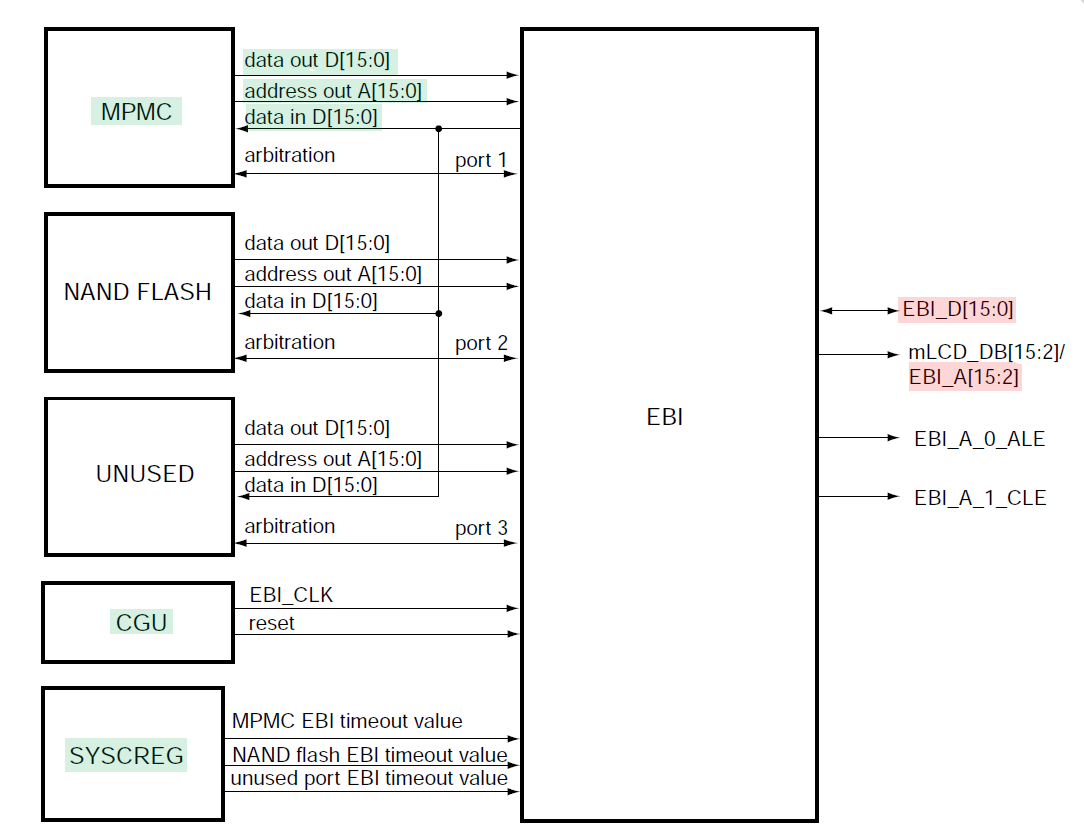
\includegraphics[width=1.0\textwidth]{TeilA/lpc_ebi.png}}
	\caption{NXP LPC313x EBI, Quelle: \cite{NXP2010}}
	\label{fig:lpc_ebi}
\end{figure}
%\end{minipage}

In \refa{fig:lpc_ebi} ist ein Blockschaltbild des EBI zu sehen, bei welchem neben CGU \footnote{CGU: Clock Generation Unit, Takterzeugung} und SYSCREG\footnote{SYSCREG: System Control Register, Steuerregister}, MPMC\footnote{MPMC: Multiport Memory Controller} sowie das NAND Flash an den Eingängen des EBI angeschlossen sind. Abgesehen von NAND Flash sind die Eingänge zum EBI für diese Arbeit relevant und grün markiert. An den Ausgängen des EBI sind Adress- und Datenbus zum Anschluss an externe Bausteine herausgeführt. Damit verschiedenartigen Bausteine an denselben Adress- und Datenpins angeschlossen werden kann, ist eine Priorisierung notwendig. Die Höchste Priorität besitzt der MPMC, gefolgt vom NAND Flash. 
Die Grundidee ist, das Display über den MPMC anzuschließen, da er so konfiguriert werden kann, dass er sich 8080-konform verhält. Die für diese Arbeit interessanten Leitungen am Ausgang des EBI sind mit rot markiert. Hier wird der Datenbus selbst, sowie die oberen 13 Bit des Adressbus gezeigt.


\subsection{MPMC - Multiport Memory Controller des NXP LPC313x}
\label{cha:mpmc}

Der MPMC stellt die Möglichkeit zur Verfügung Bausteine wie dynamisches und statisches RAM anzubinden. Die Refresh-Zyklen werden bei Verwendung von dynamischen RAMs automatisch vollzogen. Das SDRAM-Interface bietet von Haus aus die Möglichkeit Displays mit 8080-Interface zu betreiben. Dies schließt allerdings die Verwendung von dynamischen RAMs aus. Soll ein Betriebssystem wie Linux auf dem System betrieben werden, ist allerdings die Verwendung von dynamischem RAM unerlässlich. Im Folgenden wird die Schnittstelle für das statische RAM SRAM-Interface benannt. Es besteht die Möglichkeit das Interface des statischen RAM zu verwenden, um ein Display zu betreiben, da es sich so konfigurieren lässt, dass es sich wie ein 8080-Interface verhält. Damit sich die verschiedenen Slaves an Adress- und Datenbus nicht überschneiden, regelt das EBI den Zugriff auf die Busse über Chip-Select Leitungen. Am Gnublin ist eine dieser Chip-Select-Leitungen für das SRAM-Interface nach außen gelegt. Die restlichen Anschlüsse wie Write-Enable, Read-Enable, Reset sind ebenfalls herausgeführt \cite{NXP2010}. Ein Blockschaltbild des MPMC ist in \refa{fig:lpc_mpmc} zu sehen.


\begin{figure}[tbph]
%\begin{figure}[h!]
	\centering
\fbox{	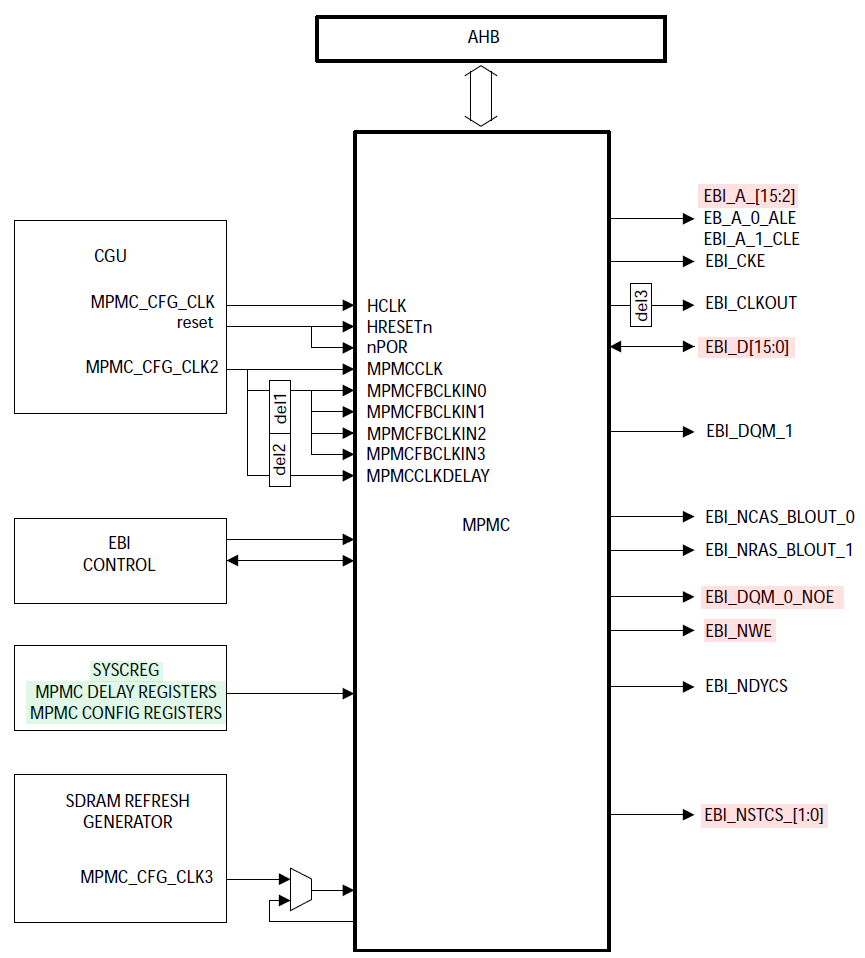
\includegraphics[width=1.0\textwidth]{TeilA/lpc_mpmc.png}}
	\caption{NXP LPC313x MPMC, \cite{NXP2010} }
	\label{fig:lpc_mpmc}
\end{figure}
\newpage
Die Register des MPMC werden so konfiguriert, dass die Schnittstelle kompatibel zum Display und dessen Timings wird. Entsprechend dem verwendeten Chip-Select-Signal werden die Register \begin{itemize}
\item MPMCStaticConfig0\item  MPMCStaticWaitWen0\item  MPMCStaticWaitOen0\item  MPMCStaticRd0\item  MPMCStaticPage0\item  MPMCStaticWr0 \item MPMCStaticWaitTurn0 \end{itemize} konfiguriert. Die Basisadresse des MPMC ist 0x1700 8000. Wie die Register zu beschreiben sind, geht aus \cite{NXP2010} auf Seite 56 hervor und ist in \reft{tab:mpmc_config} gezeigt. Die Timings wurden so gewählt, dass die Timinganforderungen der Displaycontroller eingehalten werden.

\begin{table}[h]
\begin{tabular}{|p{4cm}|p{1cm}|p{1cm}|p{6.6cm}|}\hline
\rowcolor{TableBackgroundColor} 
	\textbf{Register} 	& \textbf{Offset} 	& \textbf{Wert} & \textbf{Beschreibung} 							\\ \hline
	MPMCStaticConfig0 	& 0x200 		& 0x81 			& \begin{itemize}
	\item 16 Bit Modus \item Aktiviert die Nutzung von EBI\_nWE \item  CS low aktiv\item  keine ExtendedWait-Zyklen\item  Schreibpuffer deaktiviert\item  Geschütztes Schreiben deaktiviert \item Page Mode deaktiviert 	\end{itemize} 	\\ \hline
	MPMCStaticWaitWen0 	& 0x204 		& 13 			& 13 + 1 = 14 Wartezyklen ab Chip-Select bis Write-Enable 	\\ \hline
	MPMCStaticWaitOen0 	& 0x208 		& 0 			& 0 + 1 = 1 Wartezyklus ab Chip-Select bis Output-Enable  												\\ \hline
	MPMCStaticRd0 		& 0x20C 		& 0 			& 0 + 1 = 1 Wartezyklus ab Chip-Select bis Read-Enable					\\ \hline
	MPMCStaticPage0 	& 0x210 		& 0 			& 0 + 1 = 1 Wartezyklus für sequential Page Mode Access												\\ \hline
	MPMCStaticWr0 		& 0x214 		& 15 			& 15 + 2  = 17 Wartezyklen bis Write-Access	\\ \hline
	MPMCStaticWaitTurn0 & 0x218 		& 0 			& 0 + 1 = 1 Turnaround Cycles 								\\ \hline
\end{tabular}
\caption{MPMC Register, \cite{NXP2010}}
\label{tab:mpmc_config}
\end{table}
\newpage

Neben den MPMC-Registern muss das Register SYSCREG\_AHB\_MPMC\_MISC konfiguriert werden. Wird Bit 7 des Registers  auf der Adresse 0x1300 2864 mit dem Wert 0 eingestellt, so verändert sich das Adressierungsverhalten dahingehend, dass sich die Adressleitungen des EBI EBI\_A[15:0] auf den für den Prozessor sichtbaren AHB\footnote{AHB: Advanced Microcontroller Bus Architecture} Adressbus AHB\_A[16:1] verschiebt (siehe \cite{NXP2010}, S.~485f). Der Prozessor selbst, kann nun also 17 Bit adressieren, jedoch nur im Sprung von zwei Adressen, da das ursprüngliche LSB weggefallen ist.

\newpage
\subsection{Hardwareverbindung zwischen SRAM-Interface und Display}
In diesem Abschnitt wird die Verbindung zwischen dem Prozessor und dem Display behandelt. Eingangs wurde bereits erwähnt, dass beim Kauf der Displays Augenmerk auf Pinkompatibilität gelegt wurde. Das schlägt sich beim Entwurf der Adapterplatine positiv zu Buche, da nun lediglich ein Adapter benötigt wird. \newline
Bereits dargestellt zeigt \refa{fig:8080_pinout} auf Seite \pageref{fig:8080_pinout} das Pinout der verwendeten Displays. Der Anschluss an den Prozessor stellt sich wir in \reft{tab:display_gnublin_verbindung} dar. Anhand der gewonnenen Erkenntnisse aus \refc{cha:teila_konzept} und \refc{cha:mpmc} sowie des Schaltplans des verwendeten Gnublin Extended (siehe \cite{EmbeddedProjects2013}) kann eine Zuordnung getroffen werden. Nicht verbundene Pins sind mit 'nc'\footnote{nc: not connected} vermerkt.

\begin{table}[h]
\begin{tabular}{|p{0.6cm}|p{2.5cm}|p{2.5cm}|p{0.6cm}|p{2.5cm}|p{2.5cm}|}\hline
\rowcolor{TableBackgroundColor} 
\textbf{Nr.}	&	\textbf{Pin Display}	&	\textbf{Pin Gnublin}  & \textbf{Nr.}	&	\textbf{Pin Display}	&	\textbf{Pin Gnublin} 	\\ \hline
1				&	GND						&	GND					  &	21				&	DB0						&	LPC\_DB0				\\ \hline
2				&	+3V3					&	+3V3				  &	22				&	DB1						&	LPC\_DB1				\\ \hline
3				&	nc						&	nc				 	  & 23				&	DB2						&	LPC\_DB2				\\ \hline
4				&	RS						&	LPC\_A15	    	  &	24				&	DB3						&	LPC\_DB3				\\ \hline
5				&	WR						&	LPC\_WE				  &	25				&	DB4						&	LPC\_DB4				\\ \hline
6				&	RD						&	LPC\_DQM0			  &	26				&	DB5						&	LPC\_DB5				\\ \hline
7				&	DB8						&	LPC\_DB8			  &	27				&	DB6						&	LPC\_DB6				\\ \hline
8				&	DB9						&	LPC\_DB9			  &	28				&	DB7						&	LPC\_DB7				\\ \hline
9				&	DB10					&	LPC\_DB10			  &	29				&	nc						&	nc						\\ \hline
10				&	DB11					&	LPC\_DB11			  &	30				&	nc						&	nc						\\ \hline
11				&	DB12					&	LPC\_DB12			  &	31				&	nc						&	nc						\\ \hline
12				&	DB13					&	LPC\_DB13			  &	32				&	nc						&	nc						\\ \hline
13				&	DB14					&	LPC\_DB14			  &	33				&	nc						&	nc						\\ \hline
14				&	DB15					&	LPC\_DB15			  &	34				&	nc						&	nc						\\ \hline
15				&	CS						&	STCS0				  &	35				&	nc						&	nc						\\ \hline
16				&	nc						&	nc					  &	36				&	nc						&	nc						\\ \hline
17				&	RESET					&	GPIO19				  &	37				&	nc						&	nc						\\ \hline
18				&	nc						&	nc					  &	38				&	nc						&	nc						\\ \hline
19				&	LED-A					&	GPIO20				  &	39				&	nc						&	nc						\\ \hline
20				&	nc						&	nc				 	  &	40				&	nc						&	nc						\\ \hline

\end{tabular}
\caption{Displayverbindung mit dem Gnublin, \cite{Coldtears2014}, \cite{EmbeddedProjects2013}}
\label{tab:display_gnublin_verbindung}
\end{table}

Das Daten-Interface des Displays ist mit den Pins DB[0:15] mit dem Datenbus verbunden. Die Signale Read-Enable RD und Write-Enable WR liegen auf den Pins LPC\_DQM0 und LPC\_WE. Als Chip-Select wird das Signal STCS0 verwendet. Diese Pins sind aus dem EBI herausgeführt (siehe \refa{fig:lpc_ebi}) und werden, sofern es das System von der Auslastung am Bus ermöglicht, für das Display zur Verfügung gestellt.

Das RS Signal am Display, welches zwischen Kommando und Daten unterscheidet, liegt auf dem Adresssignal A15. Die folgenden Angaben gehen von einer Registerkonfiguration nach \refc{cha:mpmc} aus. Werden Daten gesendet, so ist der Pin logisch 1, was einem Wert auf dem Adressbus von 0x10000\footnote{0x10000 = 0b0001 0000 0000 0000 0000} entspricht. Bei Kommandos ist der Pin logisch 0 mit einem Adresswert von 0x00000\footnote{0x00000 = 0b0000 0000 0000 0000 0000}. Die unteren 16 Bits des Adressraums lassen sich also willkürlich verändern, da nur das MSB\footnote{MSB: Most Sigificant Bit, das höchstwertige Bit} vom Display verwendet wird. 

Als RS-Pin ist die Adressleitung A15 (logisch verschoben auf A16) gewählt, da so möglicherweise DMA-Transfers\footnote{DMA: Direct Memory Access, Speichertransfer effizient und schnell direkt in Hardware} von bis zu 65.536 Bytes\footnote{65.536 = $2^{16}$} möglich sind. Der DMA-Transfer könnte die Adressleitungen bei Daten von 0x10000 bis 0x1FFFF\footnote{0x1FFFF = 0b0001 1111 1111 1111 1111} bzw. bei Kommandos von 0x0000 bis 0x0FFFF\footnote{0x0FFFF = 0b0000 1111 1111 1111 1111} inkrementieren ohne die Gültigkeit der Wahl zwischen Kommando und Daten des Displays zu beeinträchtigen.

Das Display lässt sich Zusammenfassend also über zwei Pseudoregister für Kommando und Daten auf den Adressoffsets 0x00000 und 0x10000 mit der Basisadresse 0x20000000 ansprechen. Dies ist in \reft{tab:sram_adressen} nochmals übersichtlich dargestellt.

\begin{table}[h]
\begin{tabular}{|p{4.5cm}|p{4cm}|p{4cm}|}\hline
\rowcolor{TableBackgroundColor} 
	\textbf{Register} 	& \textbf{Adresse} 	& \textbf{Typ} 			\\ \hline
	SRAM0\_DISP\_CTRL 	& 0x20000000		& Kommandos				\\ \hline
	SRAM0\_DISP\_DATA 	& 0x20010000 		& Daten 				\\ \hline
\end{tabular}
\caption{Adressen für SRAM-Zugriff, \cite{NXP2010}}
\label{tab:sram_adressen}
\end{table}


Die Untersuchung inwieweit DMA-Transfer praktisch mit der verwendeten Hardware möglich ist, ist allerdings nicht Bestandteil dieser Arbeit. 

\newpage
\subsection{Adapterplatine zwischen Gnublin Extended und Display}
Der Adapter wird als Platine realisiert, die auf den Gnublin Extended aufgesteckt wird. Das Display wiederum wird mit der Adapterplatine steckbar verbunden. Der Schaltplan ist in \refa{fig:adapterplatine} gezeigt und stellt entsprechend \reft{tab:display_gnublin_verbindung} die Verbindungen her.

Der grün markierte Bereich stellt die Verbindung zum Display dar, rot zum Gnublin Extended und im blauen Rechteck sind weitere kleine Bauteile untergebracht. Hier sind Pullup-Wiederstande mit 10~k$\Omega$ an den Leitungen STCS0, Reset und LED-A um definierte Pegel vorzugeben zu sehen sowie einen Blockkondensator mit 100~nF, der für eine bessere Spannungsversorgung des Displays sorgt.

\begin{figure}[tbph]
%\begin{figure}[h!]
	\centering
\fbox{	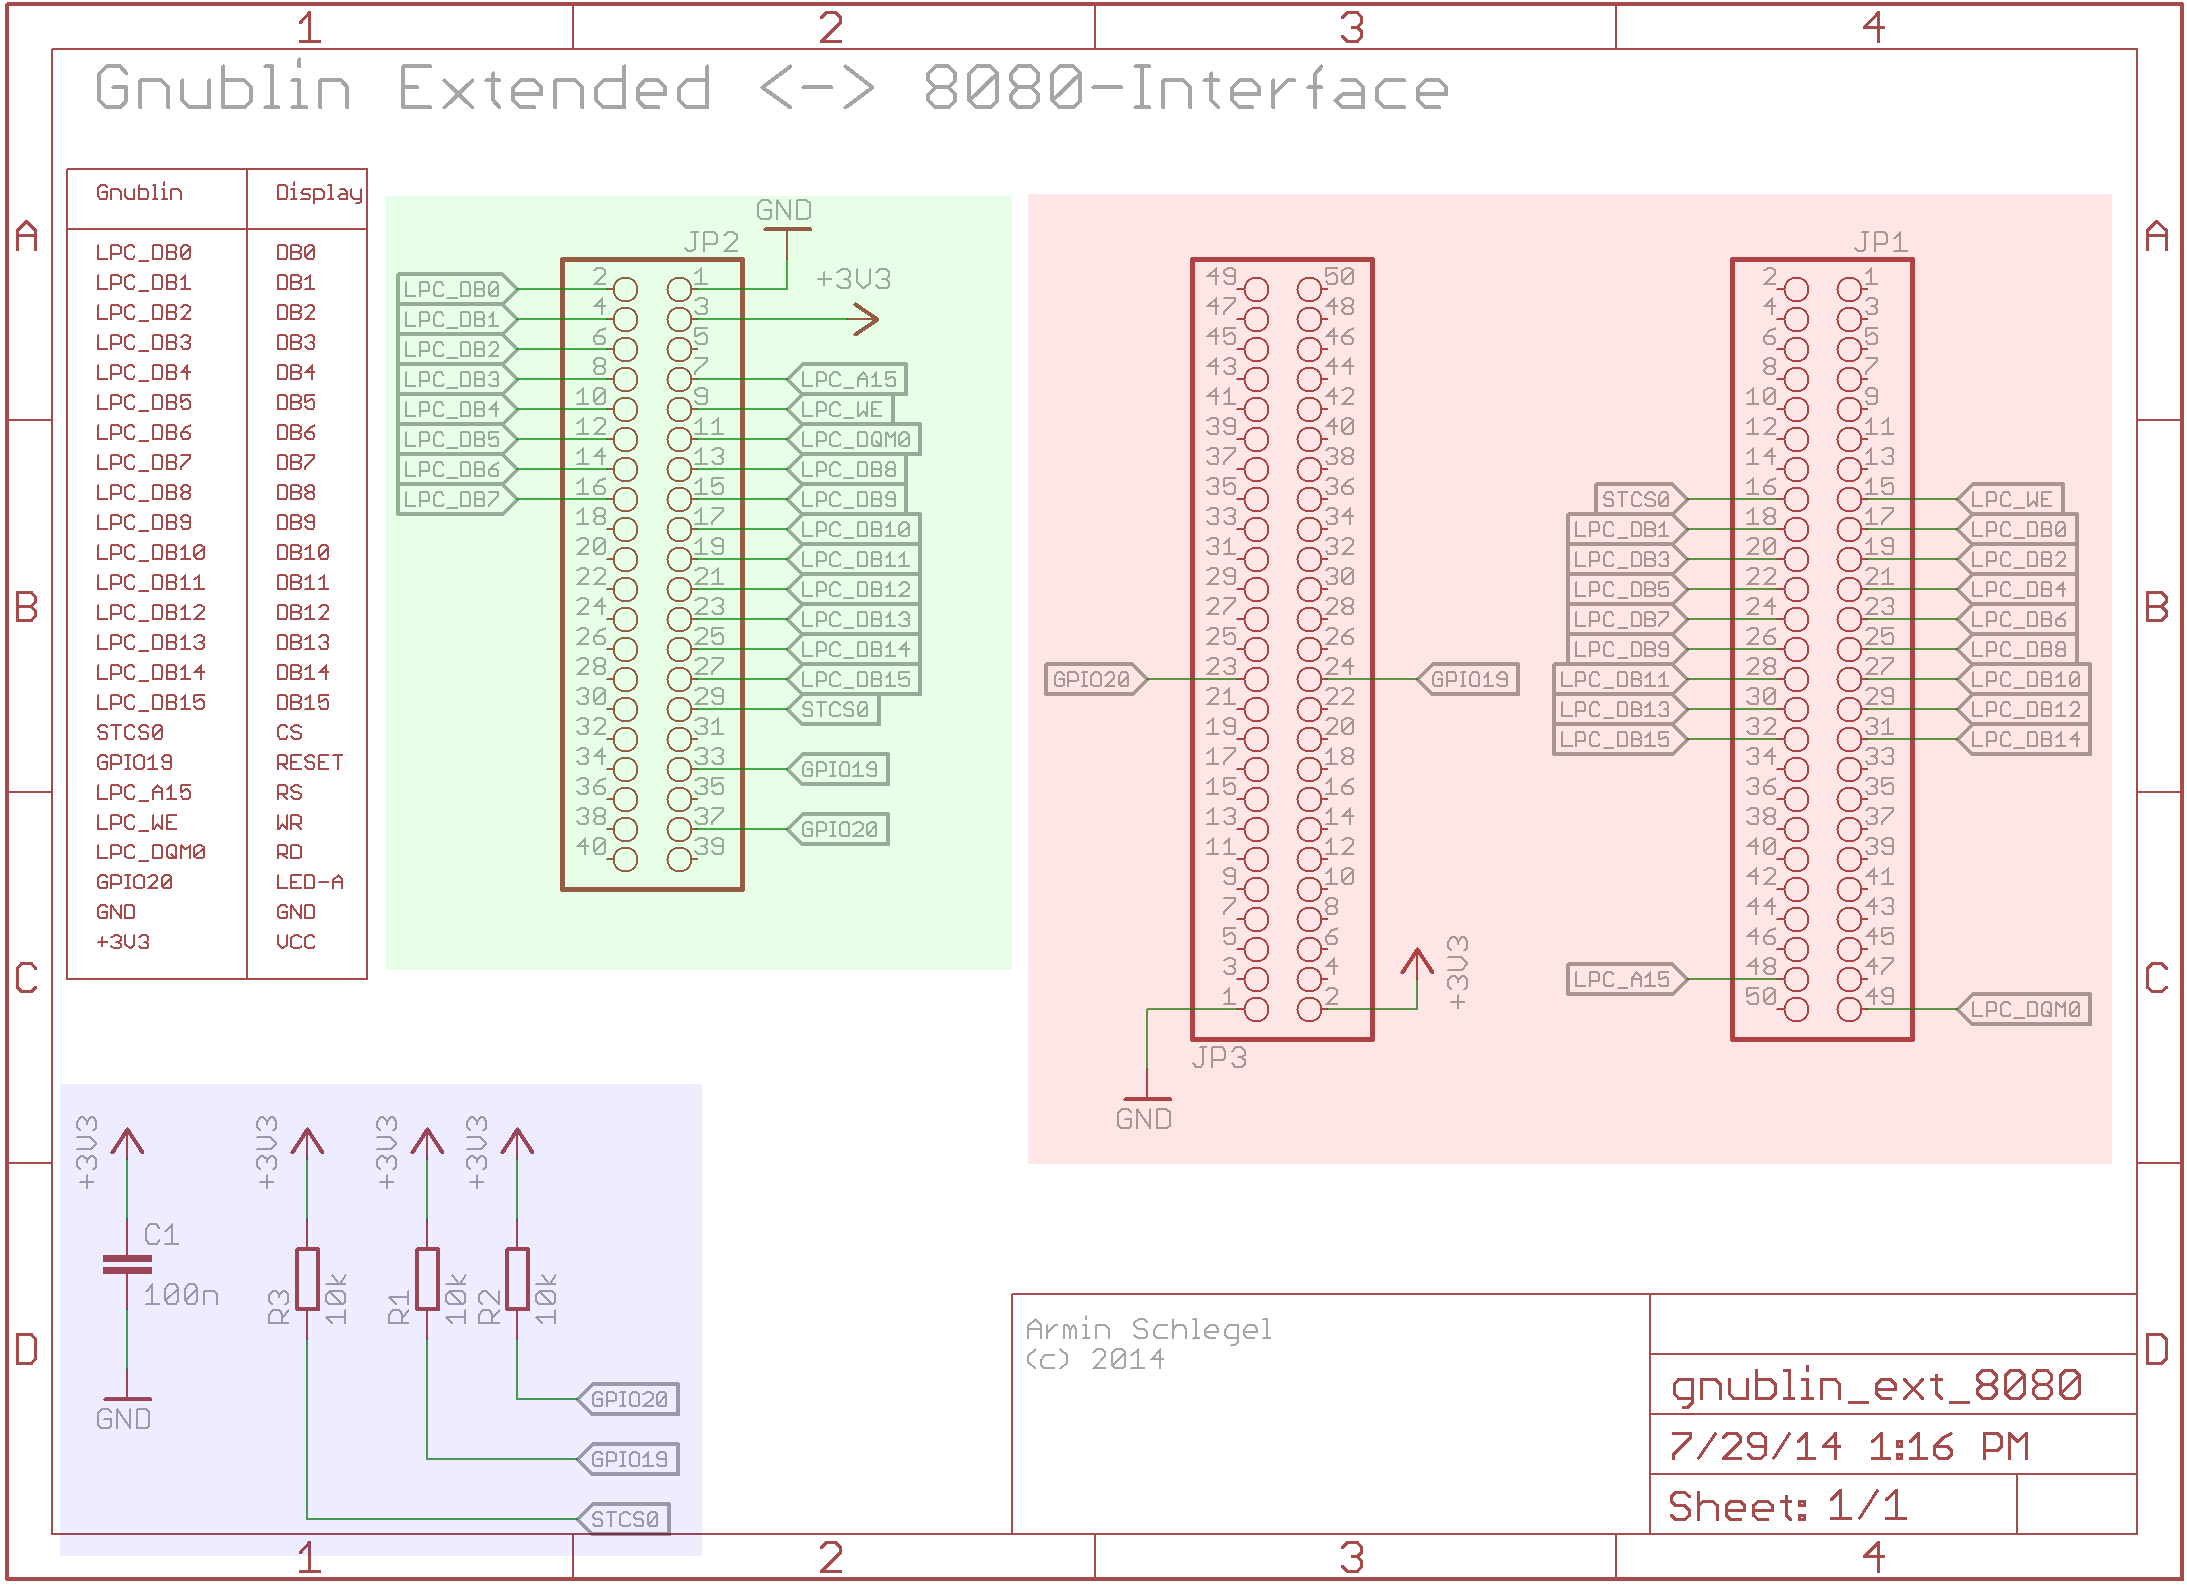
\includegraphics[width=1.0\textwidth]{TeilA/schematic.png}}
	\caption{Schaltplan Adapterplatine}
	\label{fig:adapterplatine}
\end{figure}
\newpage

\refa{fig:adapterplatine} (a) und (b) zeigt je ein gerendertes 3D Bild der Ober- und Unterseite der Adapterplatine. Auf der Oberseite wird das Display auf der linken Seite mit der 40 poligen Stiftleiste angeschossen. Mit der Unterseite wird die Platine auf das Gnublin Extended mit je zwei 50 poligen Buchsenleisten aufgesteckt.

\begin{figure}
        \begin{center}
        \begin{subfigure}[htp]{0.8\textwidth}
                \fbox{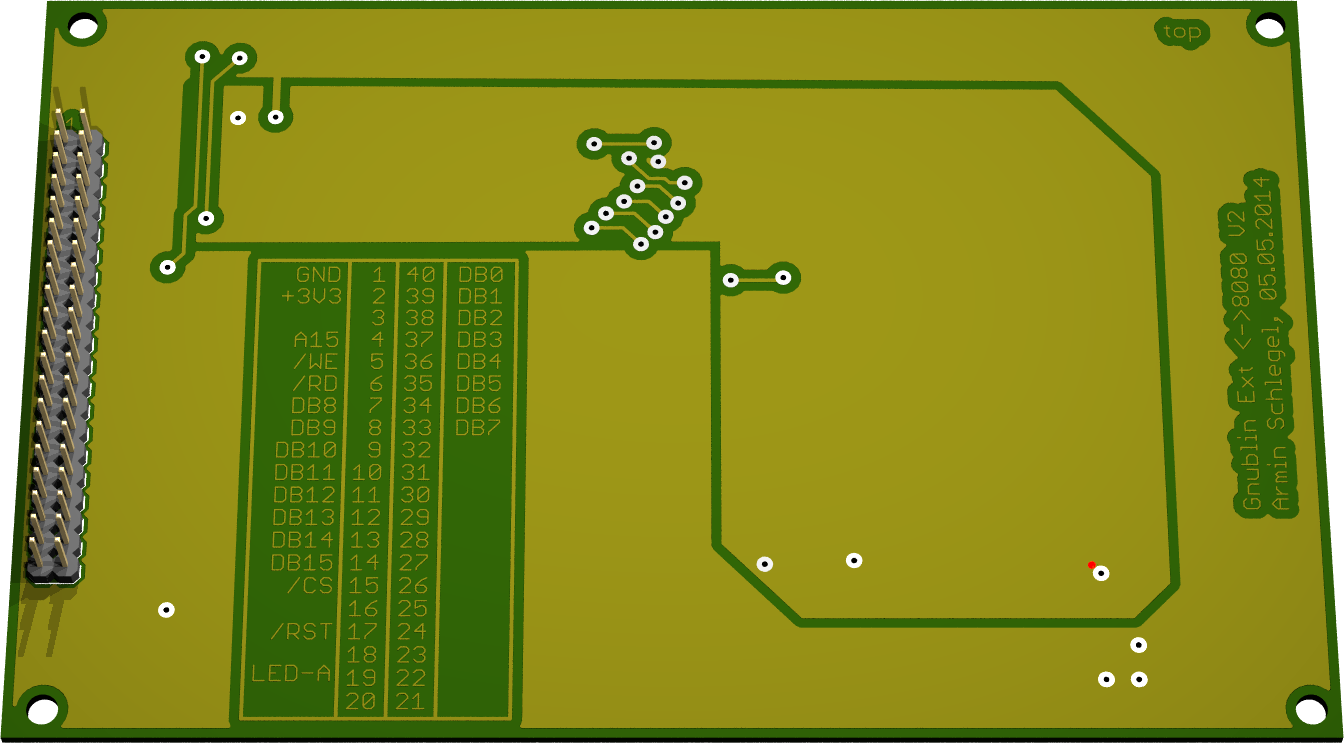
\includegraphics[width=\textwidth]{TeilA/gnublin_ext_ssd1963_top.png}}
                \caption{Adapterplatine Top Layer}
                \label{fig:adapter_top}
        \end{subfigure}

        \begin{subfigure}[htp]{0.8\textwidth}
               \fbox{ 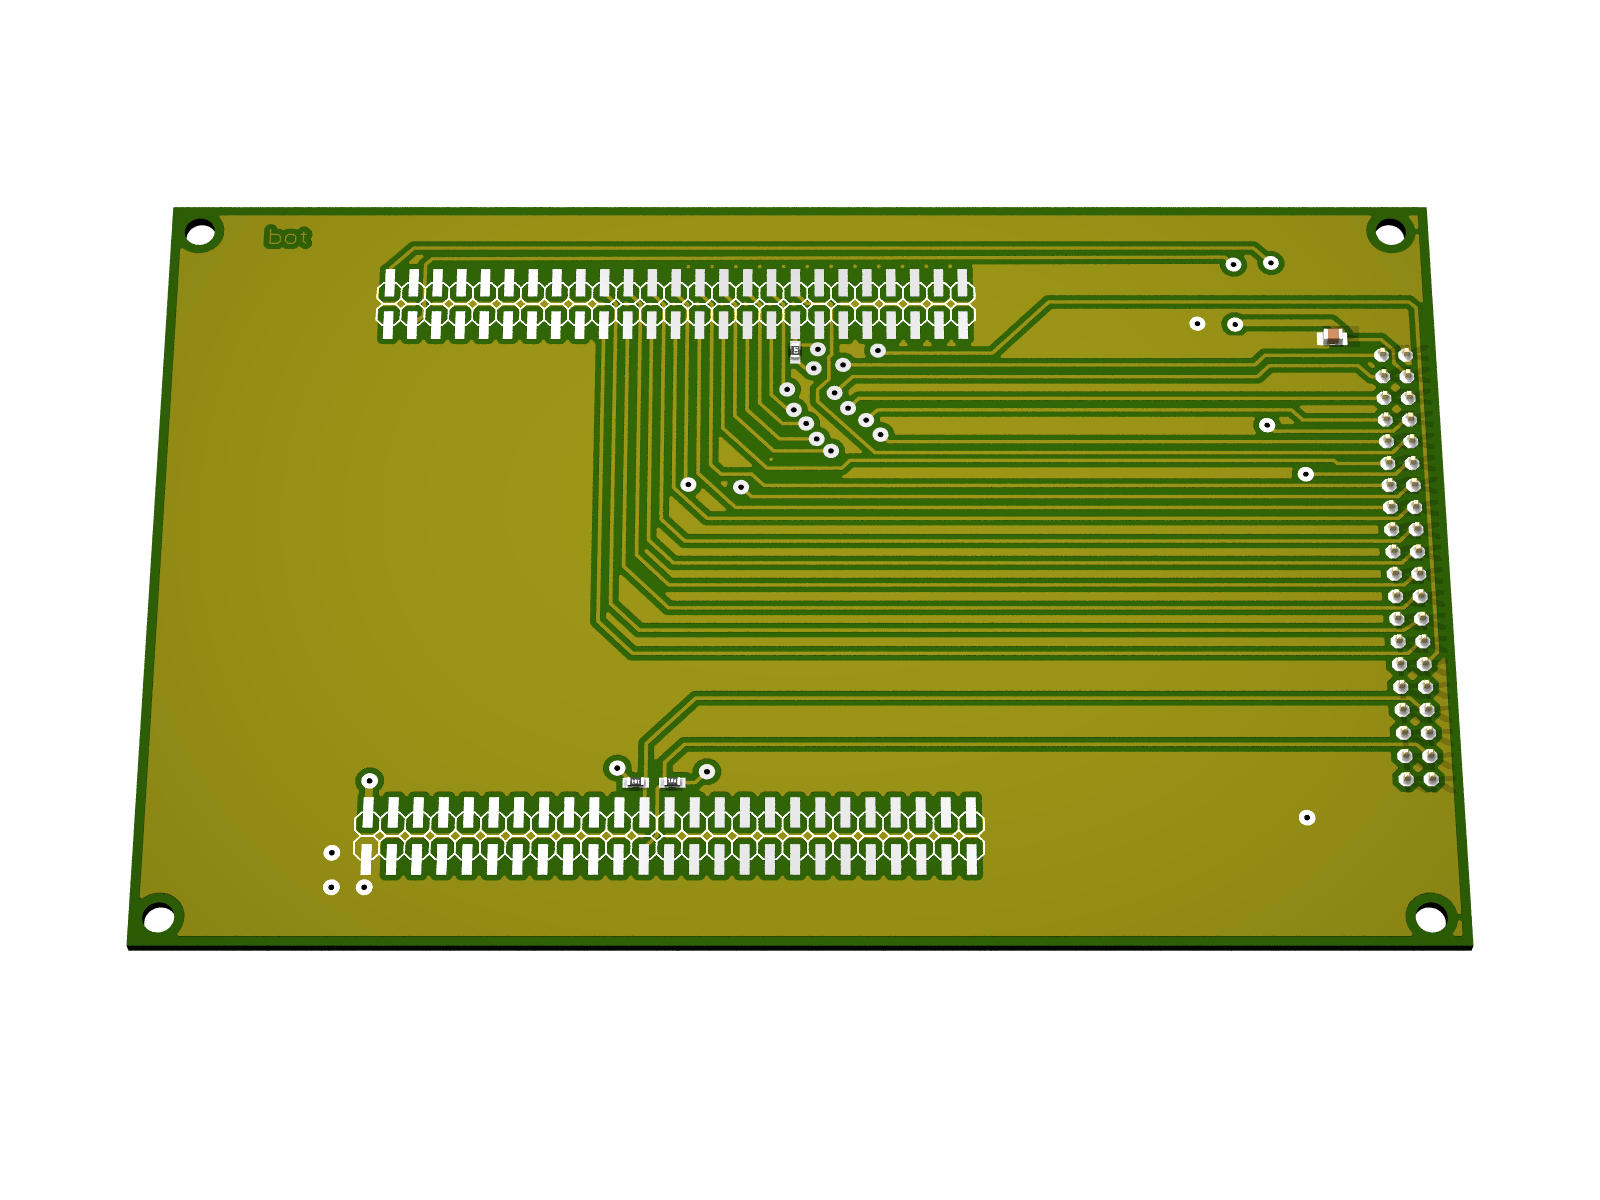
\includegraphics[width=\textwidth]{TeilA/gnublin_ext_ssd1963_bot.png} }              				\caption{Adapterplatine Bottom Layer}
                \label{fig:adapter_bot}
        \end{subfigure}
		\end{center}
        \caption{Adapterplatine zwischen Gnublin Extended und Display}\label{fig:adapterplatine}
\end{figure}

Die Schaltplan und das Layout befinden sich in der CD im Anhang dieser Arbeit.
\newpage
\subsection{Software}
Im Folgenden Abschnitt wird die Software behandelt, die nötig ist, um das Display zu betreiben. 
Die Softwareentwicklung ist in drei Teile auf gegliedert:
\begin{itemize}
\item Modifikationen im Bootloader APEX
\item Userspace-Treiber basierend auf einem Treibers auf für den Raspberry Pi (siehe \cite{Schlegel2013a} und \cite{Schlegel2013b}) bei dem mittels GPIO-Pins ein 8080-Display zu betreiben
\item Framebuffer-Treiber im Linux-Kernel
\end{itemize}

\subsubsection{Anpassung des APEX-Bootloaders zur Verwendung des Displays}
Der APEX-Bootloader\footnote{\url{https://gitorious.org/apex/}} wurde ursprünglich für Prozessoren de Sharp LH Familie entwickelt, wurde allerdings auf eine Vielzahl von weiteren ARM basierten Prozessoren portiert, so auch für die verwendeten NXP LPC313x CPU\footnote{CPU: Central Processing Unit, Prozessor}.
Die Aufgabe des Bootloaders ist es, grundlegende prozessorinterne Hardwareeinheiten wie z.b. CGU oder SD-RAM zu initialisieren um für den Linux-Kernel die notwendige Umgebung zu schaffen. Im Anschluss wird der Linux-Kernel geladen und gestartet. An dieser Stelle werden die verwendeten MPMC-Register konfiguriert. Wie in \ref{cha:mpmc} muss das SYSCREG-Register SYSCREG\_AHB\_MPMC\_MISC nicht explizit beschrieben werden, da es im Resetzustand bereits richtig konfiguriert wird. 
\paragraph{Boot-Logo im APEX-Bootloader}
Um dem Display beim Systemstart einen initialisierten Zustand zu geben und dem Benutzer bereits während des Ladens des Linux-Kernels ein Bild zu anzuzeigen, ist ein Bootlogo konfigurierbar. Hierfür bedarf es einem Displaytreiber im Bootloader. Im Folgenden wird die Darstellung des Boot-Logos unter Verwendung des CPLD-basierten Displays dargestellt. \refl{lst:apex_gemeinsamer_teil} zeigt den gemeinsamen Teil des Treibers, bei dem grundlegende Datentypen sowie Sendefunktionen für Daten und Kommandos gelistet sind. 

\begin{lstlisting}[%
language=MyC,
caption={Funktionen zum Senden und grundlegende Datentypen fuer den Treiber},
label=lst:apex_gemeinsamer_teil
]
#if defined(CONFIG_DISP_MD050SD) || defined(CONFIG_DISP_SSD1963) || defined(CONFIG_DISP_SSD1289)
#define DISP_PHYS        (EXT_SRAM0_PHYS)
#define DISP_PHYS_CTRL   (DISP_PHYS + 0)
#define DISP_PHYS_DATA   (DISP_PHYS + 0x10000)

unsigned int width;
unsigned int height;
int pixel;

struct display {
   volatile u16* ctrl;
   volatile u16* data;
};

static struct display display;

static void display_send_cmd(u16 cmd)
{
   *display.ctrl = 0x00FF & cmd;
}

static void display_send_data(u16 data)
{
   *display.data = data;
}

#endif
\end{lstlisting}

Die Struktur \todo{code style?} display in Zeile 10 von \refl{lst:apex_gemeinsamer_teil} enthält Zeiger auf die jeweiligen Adressen aus \reft{tab:sram_adressen}. 


\begin{lstlisting}[%
language=MyC,
caption={
Display Initialisierung und Logo},
label=lst:apex_init_und_logo
]
#if defined(CONFIG_DISP_MD050SD) || defined(CONFIG_DISP_SSD1963) || defined(CONFIG_DISP_SSD1289)
   display.ctrl = &__REG16 (DISP_PHYS_CTRL);   
   display.data = &__REG16 (DISP_PHYS_DATA); 
#if defined(CONFIG_DISP_MD050SD)
   GPIO_OUT_LOW(IOCONF_GPIO, _BIT(14)); //GPIO20 is LED_ENABLE

   GPIO_OUT_LOW(IOCONF_GPIO, _BIT(13)); //GPIO19 is nRESET
   udelay(20000);
   GPIO_OUT_HIGH(IOCONF_GPIO, _BIT(13)); //GPIO19 is nRESET
   udelay(20000);

	/* Set Window from 0,0 to 479, 799 */
   display_send_cmd(0x0002);			
   display_send_data(0);				
   display_send_cmd(0x0003);			
   display_send_data(0);				

   display_send_cmd(0x0006);
   display_send_data(480 - 1);
   display_send_cmd(0x0007);
   display_send_data(800 - 1);

	/* Clear the display with color black */
   display_send_cmd(0x000F);

   for(pixel = 0; pixel <= 800 * 480; pixel++)
   {
      display_send_data(0x0000);
   }

   GPIO_OUT_HIGH(IOCONF_GPIO, _BIT(14)); //GPIO20 is LED_ENABLE

#if defined(CONFIG_LOGO_TUX)
   width = boot_logo_tux[0];
   height = boot_logo_tux[1];

   display_send_cmd(0x0002);
   display_send_data(480/2 - (height - 1)/2);
   display_send_cmd(0x0003);
   display_send_data(800/2 - (width - 1)/2);
   display_send_cmd(0x0006);
   display_send_data(480/2 + (height - 1)/2 + 1);
   display_send_cmd(0x0007);
   display_send_data(800/2 + (width - 1)/2 + 1);
   display_send_cmd(0x000F);

   for(pixel = 2; pixel < width * height + 2; pixel++)
   {
      display_send_data(boot_logo_tux[pixel]);
   }
#endif
#endif
#endif
\end{lstlisting}




\paragraph{Konfiguration des APEX-Bootloaders}


\paragraph{Inbetriebnahme des APEX-Bootloaders}




\subsubsection{Entwicklung eines Linux-Framebuffer-Treibers}
\paragraph{Anpassungen für SSD1963 Controller}
\paragraph{Anpassungen für SSD1289 Controller}
\paragraph{Anpassungen für CPLD Controller}
\subsubsection{Entwicklung eines User-Space-Treibers}
\paragraph{Anpassungen für SSD1963 Controller}
\paragraph{Anpassungen für SSD1289 Controller}
\paragraph{Anpassungen für CPLD Controller}
\subsubsection{Probleme bei der Entwicklung und Fehlersuche}
\paragraph{Probleme mit SSD1963}
\subparagraph{Rolle des User-Space-Treibers}
\subparagraph{Debuggen mit Logik-Analyzer}



